\section{Methodology}
\label{sec:methodology}
RGB images depict objects based on color differences that match human perception. However, objects with similar colors may not have enough color contrast to show their shape. By contrast, polarized light is strongly linked to the material of objects and the orientation of the reflecting surface, enabling it to reveal material properties that make object boundaries visible even when colors are similar (\textit{e.g.}, Fig. \ref{fig:samples} (a) and (b)). In spite of that, polarization cues may be weak in certain lighting conditions or viewing angles (\textit{e.g.}, Fig. \ref{fig:samples} (c)). Including polarization measurements naively in existing car detection methods may not necessarily yield the expected performance improvement. How to effectively integrate RGB and polarization features is a key challenge to be addressed to achieve robust car detection.

We introduce a novel Polarization Car Detection Network (PCDNet) that is capable of exploring and integrating polarized material cues for robust car detection. As shown in Fig. \ref{fig:pipeline}, PCDNet takes as input the RGB intensity, trichromatic AoLP and DoLP, and outputs car detections. The AoLP and DoLP are first integrated into a comprehensive and semantically meaningful polarization feature representation by a Polarization Integration (PI) module for the ease of the following feature extraction and fusion. Then, the RGB and polarization features are separately fed into two branches of CSPDarkNet \cite{wang2020cspnet} encoder, each consisting of five stages to extract multi-level contextual features. The Material Perception (MP) module, which aims to extract the intrinsic material properties of cars across the whole learning samples, is applied to different levels of extracted features. The MP module has a specific design for low-level features (MSP with spatial specialization) and high-level features (MCP with channel specialization), respectively. For multimodal feature fusion, the Cross-Domain Demand Query (CDDQ) module assigns fusion weights adaptively and conducts dynamic fusion in a request-and-complement manner. Finally, based on the fused features, we adopt the anchor-based detection head from YOLOv7 \cite{wang2022yolov7} to generate final classifications and bounding boxes.

\subsection{Polarization Integration (PI)}
AoLP $\phi$ and DoLP $\rho$ reveal object/scene materials from two different aspects. Polarization Integration (PI) module is designed to combine them into an unified and semantically meaningful polarization representation $F_{pol}$ for the ease of the following feature extraction and fusion. As the captured polarization angle is more likely random at regions with a low polarization degree, PI filters the AoLP measurement based on the DoLP. In addition, PI also extracts and integrates the edge information in DoLP measurement to help the distinction of objects with different materials. Formally,
\begin{align} \label{eq:pim}
    F_{pol} &=\vartheta_{3\cdot 1}([\vartheta_{3\cdot 1}(F_{\phi\rho}), \vartheta_{3\cdot 1}(\rho+\mathbb{E}(\rho))]), \\
    F_{\phi\rho} &=\phi\otimes(\vartheta_{3\cdot 1}([\hat{\mathbb{A}}(\rho),\hat{\mathbb{M}}(\rho)])+\sigma(\mathbb{M}(\vartheta_{3\cdot 1}(\rho)))),
\end{align}
where $\vartheta_{k\cdot s}$ denotes a $k \times k$ convolution with a stride of $s$, followed by a batch normalization and a SiLU activation function. $[\cdot]$ indicates the concatenation operation over the channel dimension. $\mathbb{E}$ refers to the Scharr edge extractor. $\otimes$ is the element-wise multiplication. $\hat{\mathbb{A}}$ and $\hat{\mathbb{M}}$ are the average and max pooling in the channel dimension, respectively. $\mathbb{M}$ is the max pooling in the spatial dimension with a kernel size of 5. And $\sigma$ is the Sigmoid activation.

\subsection{Material Perception (MP)}
Despite the cars in different scenarios may have diverse visual appearances such as different colors and textures, they are typically share similar materials including glass, rubber, metal, etc. Fortunately, polarization can robustly reveal the intrinsic physical properties of these materials. Inspired by this, we design the Material Perception (MP) strategy to explore
% and memorize 
the discriminative and invariant material features of cars across different scenarios. Considering the different characteristics of different levels of features, \textit{i.e.}, low-level features have larger spatial sizes and keep rich and detailed low-level information while high-level features contain more semantic cues distributed in more feature channels, MP is instantialized as Material Spatial/Channel Perception (MSP/MCP) modules for the low-/high-level polarization features, respectively. Formally, MSP/MCP can be described as:
\begin{align} \label{eq:mpm}
    MSP(F) &=\varrho_{2\cdot2}(\varrho_{2\cdot2}(\vartheta_{3\cdot2}(\vartheta_{3\cdot2}(F)))), \\
    MCP(F) &=\varrho_{2\cdot2}(\mathcal{M}((\vartheta_{1\cdot1}(\vartheta_{3\cdot2}(F))))), \\
    \mathcal{M}(x) &=x+x\otimes\sigma(m_2(m_1(\bar{\mathbb{A}}(x)))),
\end{align}
where $\varrho_{k\cdot s}$ denotes a $k \times k$ transposed convolution with a stride of $s$, followed by a batch normalization and a SiLU activation function. $\mathcal{M}(\cdot)$ is the perception scheme with two independent perception matrices in fully connected layers named $m_1$ and $m_2$. And $\bar{\mathbb{A}}$ is global average pooling.

\subsection{Cross Domain Demand Query (CDDQ)}
Polarization and RGB features are different types of representations of the scenes and simply combing them may dilute the useful clues of the cars originally presented in the individual modality or amplify the background interference. We address this issue by introducing the Cross-Domain Demand Query (CDDQ) module for effective multimodal feature fusion, taking into account both the context and quality of each modality feature. CDDQ takes as input the RGB features $F_{rgb}$ and polarization representations $F'_{pol}$. It first utilizes a Spatial Demand Map Delivery (SDMD) block to generate enhanced RGB features $F_{rgb}^{*}$ and distill informative and required polarization features $F_{pol}^{*}$ and then obtains fused features $F_{fused}$ through a Channel Weight Dynamic Assignment (CWDA) block:
\allowdisplaybreaks\begin{align}
    F_{rgb}^{*} &=F_{rgb}+F''_{rgb} = F_{rgb}+\mu\otimes F'_{rgb} \nonumber \\
        &=F_{rgb}+\mu\otimes \eta\otimes F_{rgb}, \\
    \eta &=\sigma(\vartheta_{1\cdot1}(\bar{\mathbb{M}}(F_{rgb}))+\vartheta_{1\cdot1}(\bar{\mathbb{A}}(F_{rgb}))), \\
% \end{align} 
% \begin{align}
    \mu &=\sigma(\vartheta_{7\cdot1}([\hat{\mathbb{A}}(F'_{rgb}), \hat{\mathbb{M}}(F'_{rgb})])), \\
    F_{pol}^{*} &=F'_{pol}+\vartheta_{3\cdot1}(\mathbb{A}(\mu))\otimes F'_{pol}, \\
    F_{fused} &=\vartheta_{1\cdot1}([\alpha\times F_{rgb}^{*},\beta\times F_{pol}^{*}]), \\
    \alpha, \beta &=\delta(\langle\sigma(fc(si(fc([\bar{\mathbb{A}}(F_{rgb}^{*}), \bar{\mathbb{A}}(F_{pol}^{*})]))))\rangle),
\end{align}
where $\eta$ is the channel attention vector. $\mu$ is the spatial attention map which also serves as the guidance of the informative polarization cues request process. $\mathbb{A}$ is an average pooling with a kernel size of 3. $\bar{\mathbb{M}}$/$\bar{\mathbb{A}}$ denotes global max/average pooling. $\alpha$ and $\beta$ are dynamic fusion weights assigned to the RGB and polarization features, respectively, with a constraint of being non-negative and summing up to 1 for each channel position. $fc$ is the fully connected layer and $\langle\cdot\rangle$ is the split operation over the channel dimension. $si$ and $\delta$ are the SiLU and Softmax activation functions, respectively.

\begin{figure}[ht]
    \begin{center}
        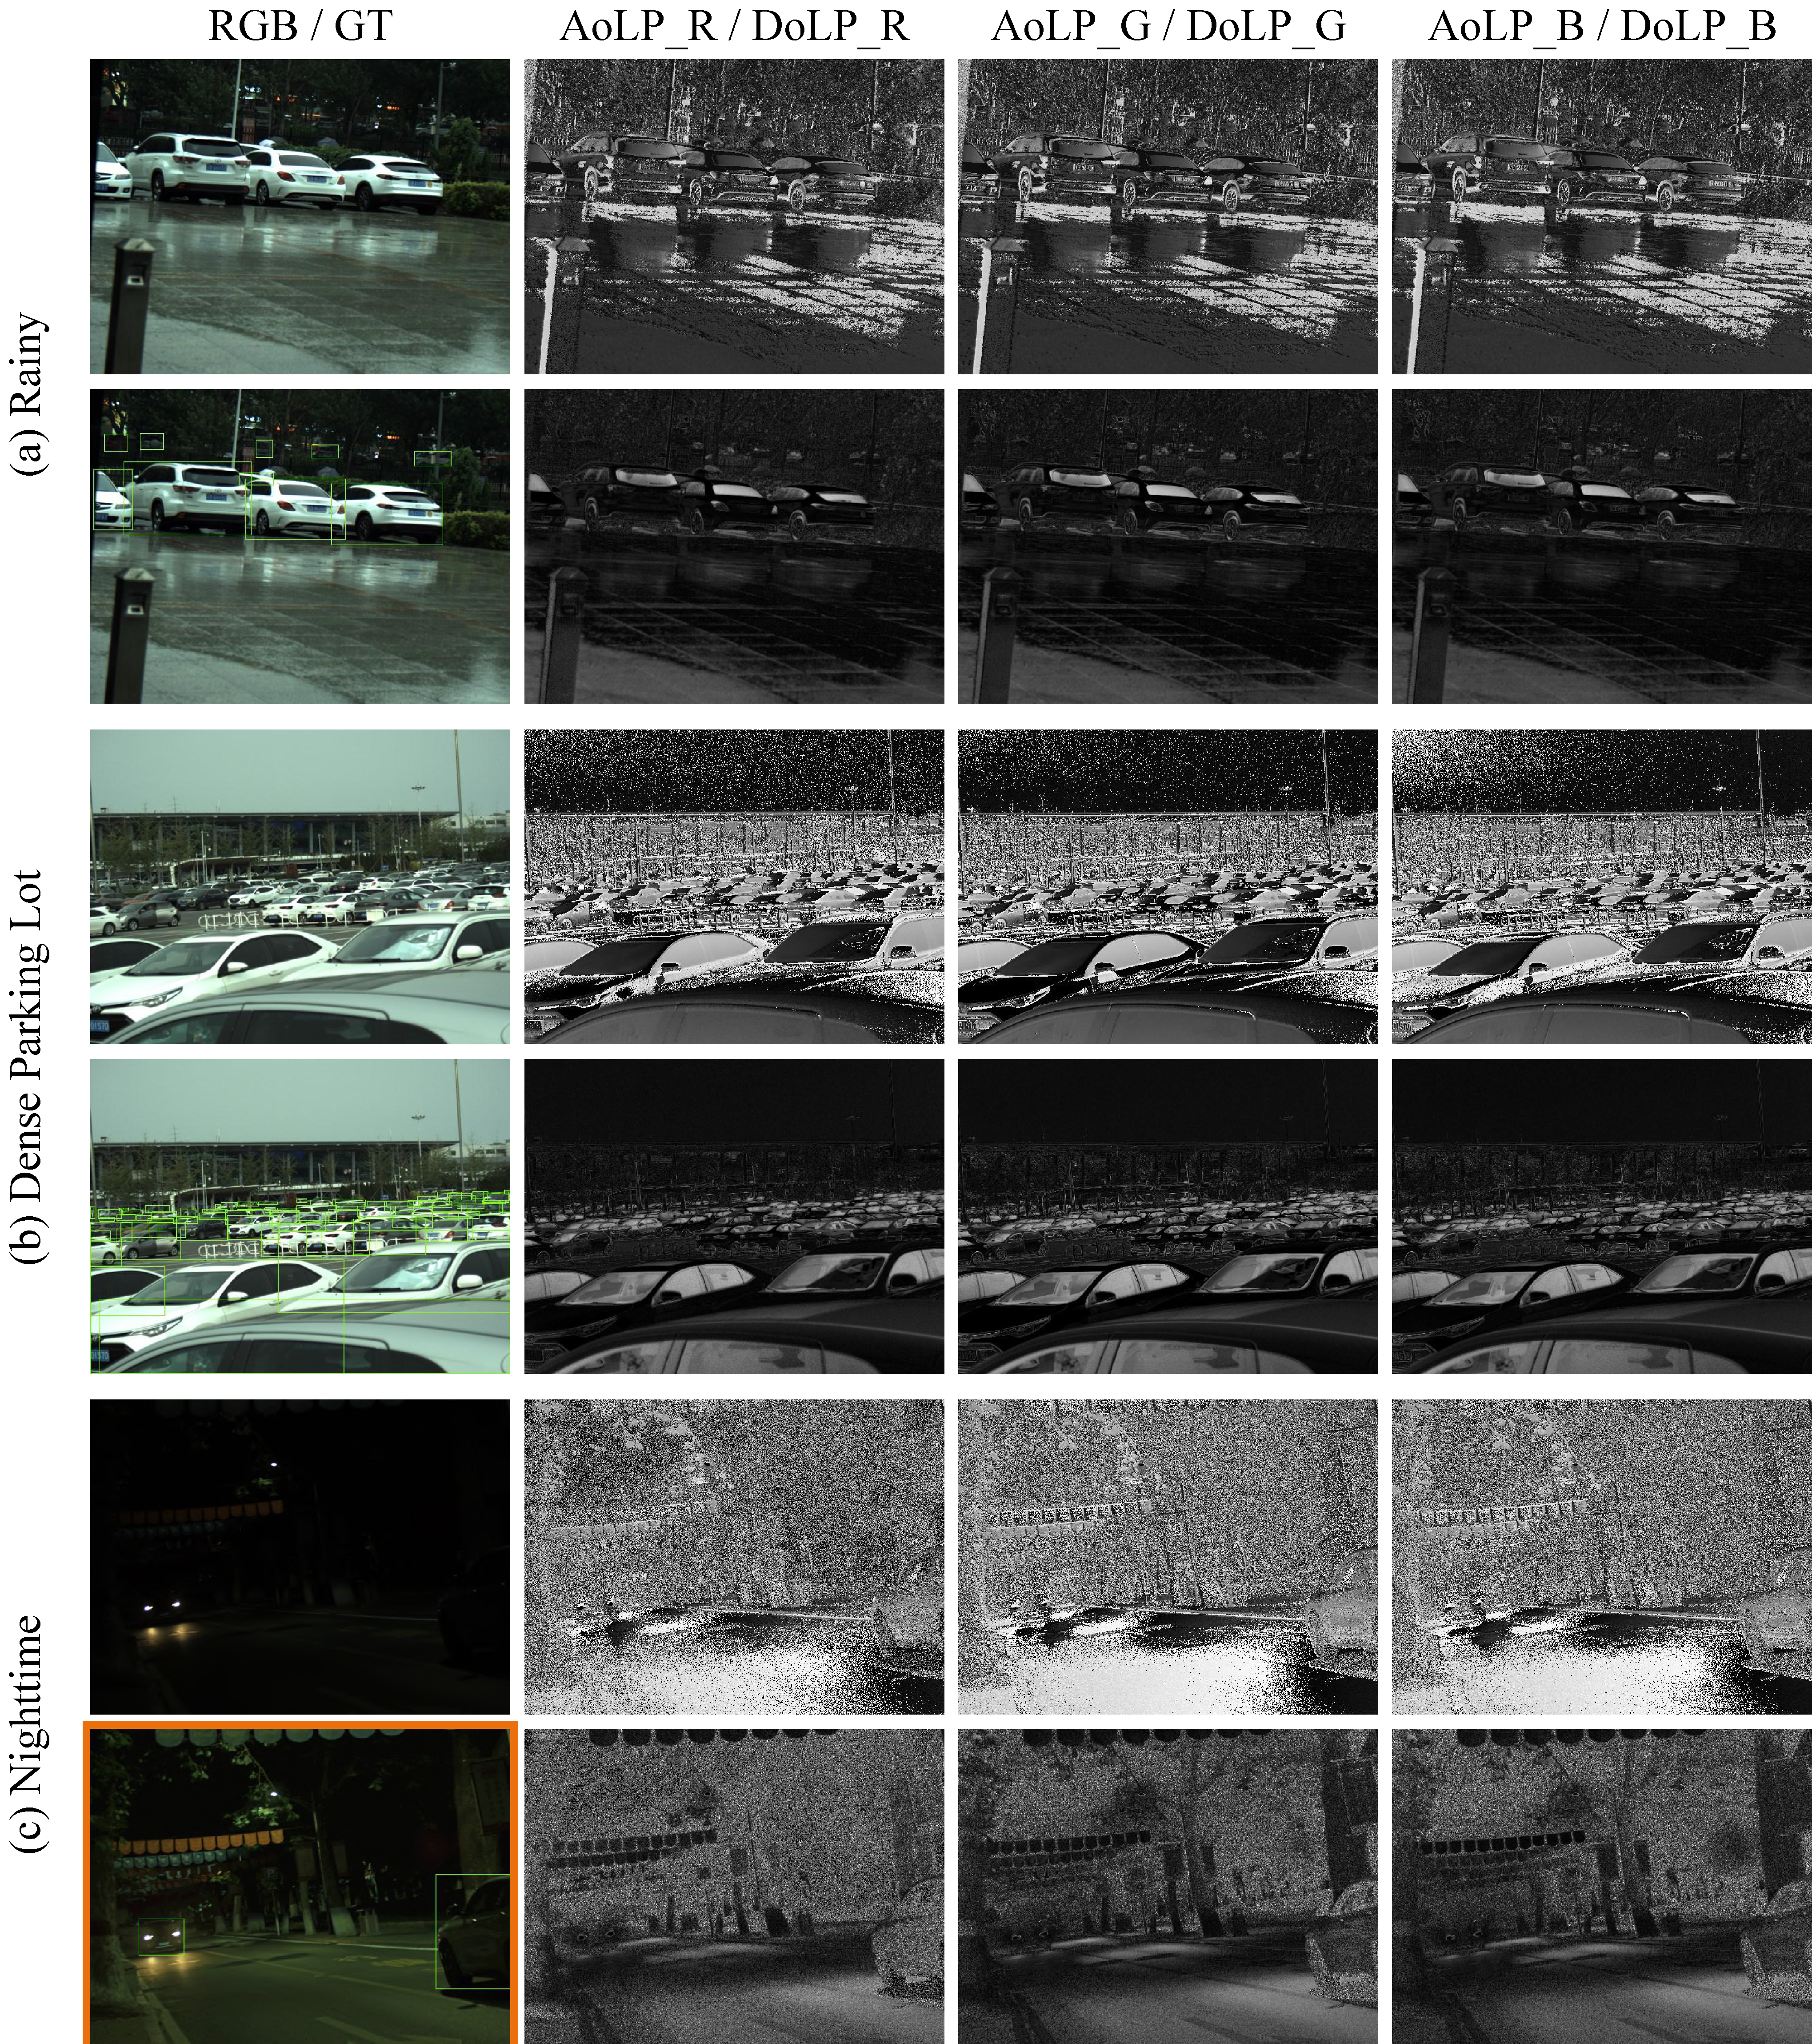
\includegraphics[width=1\linewidth]{figure/dataset.pdf}
    \end{center}
    \caption{
    RGBP-Car Examples. The first column displays the RGB intensity (top) and the corresponding annotation (bottom). The next three columns show the AoLP (top) and DoLP (bottom) measurements for the red, green, and blue channels, respectively. From top to bottom are scenes of stopped cars in a rainy parking lot, dense cars in an outdoor parking lot, and driving cars on a clear night road, respectively. 
    (The low-light RGB image is enhanced by ZeroDCE \cite{guo2020zero} (with \orange{orange} frame) for visualization.)}
    \label{fig:samples}
\end{figure}
